% !TEX root = ../../seminar.tex

\subsection{Answer Question}
\label{subsec:answer question}

Before you can answer a question the existing studies must be critically appraised. This means checking the study design, study quality, relevance for the research question, as well as consistency between different studies. 

Rainer \etal found that \q{students use limited criteria for identifying the best or better evidence} \cite{Rainer2006} (see issue \ref{itm:issue2} in table \ref{table:issuesEBSE}). They suggest sensitizing students for biases to solve this issue. We also suggest guiding the user through the process, because students had additional problems (see issue \ref{itm:issue6}). \todosoft{rephrase}

The \emph{GRADE approach} \cite{Atkins2004} is a grading system for studies that goes beyond simple hierarchies of study types. It was introduced for medicine and has been used in the software engineering domain \cite{Wohlin2013EvidenceProfile,Dyba2008}. It is a well-defined method and differentiates between the quality of evidence and the strength of recommendation. Figure \ref{fig:critical appraisal} shows a checklist containing the important factors to consider when appraising a study and we suggest following it when appraising studies. \todo{ref issue \ref{itm:issue6} in table \ref{table:issuesEBSE}}

\begin{figure}
	\centering
	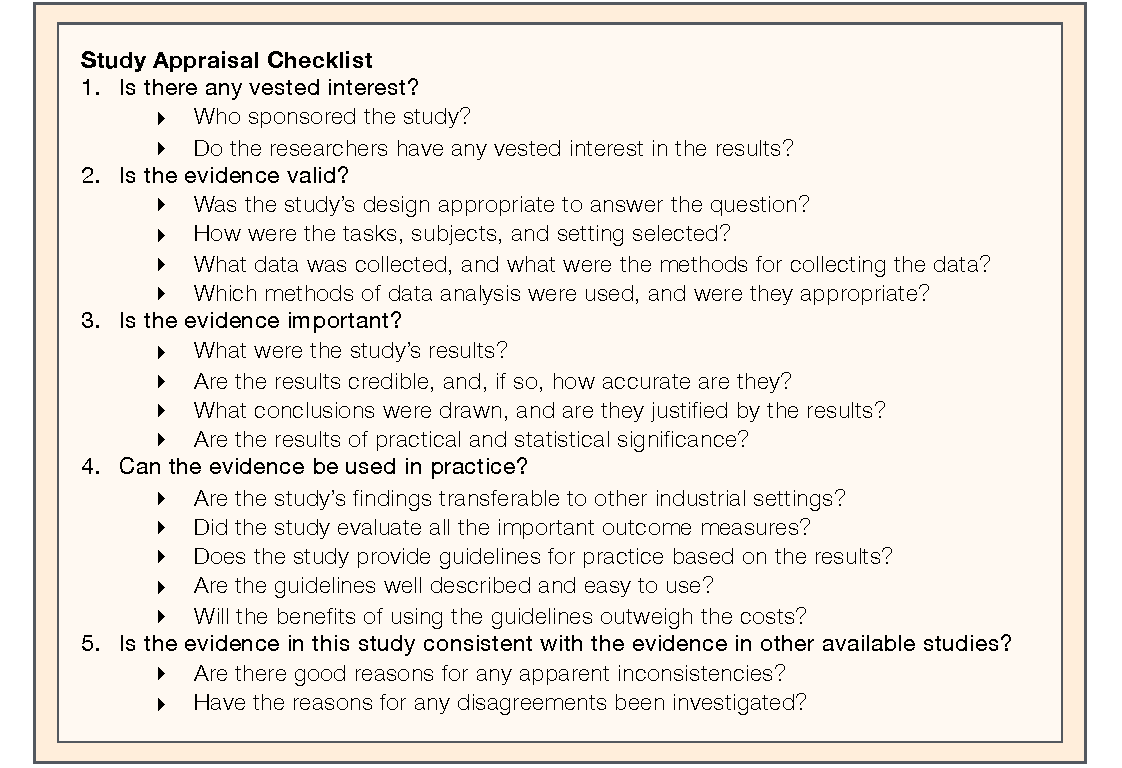
\includegraphics[width=12cm]{figures/study_appraisal.pdf}
\caption{Checklist for critical appraisal of studies compiled by Dyb{\aa} \etal \cite{Dyba2005} \todo{image}}
\label{fig:critical appraisal}
\end{figure}

One important aspect of appraising studies is checking whether they might be biased. J{\o}rgensen \etal \cite{Jorgensen2016} reported indications of research and publication bias being quite common in the domain of software engineering. Shepperd makes similar findings and gives a good and short overview of the problem \cite{Shepperd2015}.

The hypothesis is accepted or rejected on the basis of the critical appraisal and the research question is answered accordingly.


\todosoft{- maybe reference to different types of bias}
